\newpage
\chapter{Missing mass distributions}
\label{ch:mm}
\mbox{}\vspace{-\baselineskip}

Let's consider a sample of events that correspond to the reaction of double-pion electroproduction off protons $ep\rightarrow e'p'\pi^{+}\pi^{-}$. Then the following missing quantities can be defined,
\begin{equation}
\begin{aligned}
&M_{X[0]}^{2}&=&\left [P_{X[0]}^{\mu} \right ]^{2}&=&~\left (P_{e}^{\mu} + P_{p}^{\mu}- P_{e'}^{\mu}- P_{p'}^{\mu}-  P_{\pi^{+}}^{\mu} - P_{\pi^{-}}^{\mu}\right )^{2}~~\textrm{and}\\
&M_{X[\pi^{-}]}^{2}&=&\left [P_{X[\pi^{-}]}^{\mu}\right ]^{2}&=&~\left (P_{e}^{\mu} + P_{p}^{\mu}- P_{e'}^{\mu}- P_{p'}^{\mu}-  P_{\pi^{+}}^{\mu}\right )^{2},\\
\end{aligned}\label{eq:mm_def}
\end{equation}
where $P_{X[0]}^{\mu}$ and $P_{X[\pi^{-}]}^{\mu}$ are the corresponding missing four-vectors, while $P_{i}^{\mu}$ is the four-momentum of the particle $i$.



Let's first assume that (i) the target proton is free and at rest, (ii) no events from other channels are present in the sample, (iii) all four-momenta $P_{i}^{\mu}$ are defined exactly without any uncertainty, and (iv) neither radiative effects nor FSI occur. 

\begin{figure}[htp]
\begin{center}
\framebox{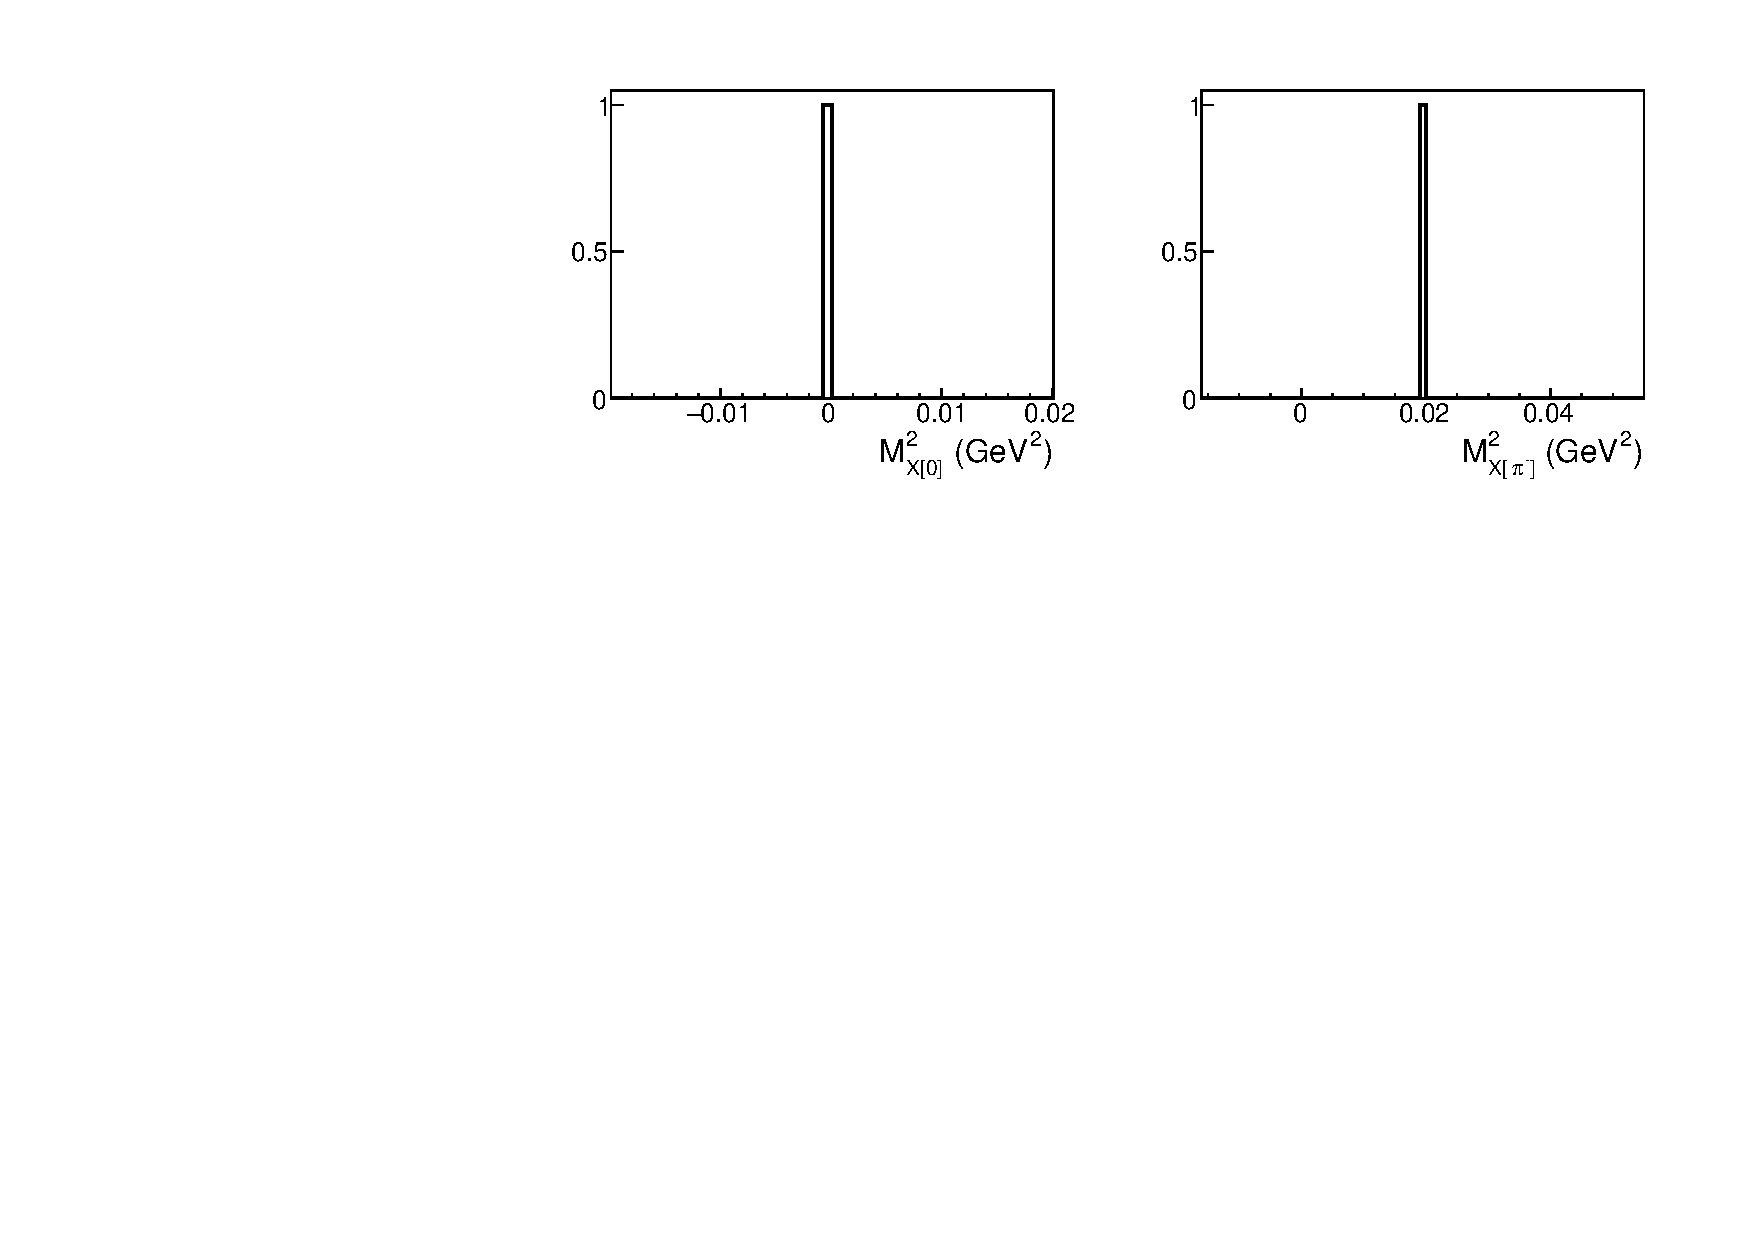
\includegraphics[width=\textwidth]{pictures/mm_norad_nofsi.pdf}}
\caption{\small Simulated distributions of the quantities $M_{X[0]}^{2}$ (left) and $M_{X[\pi^{-}]}^{2}$ (right) plotted under the assumptions specified in the text.} \label{fig:norad_nofsi}
\end{center}
\end{figure}


Then, using energy-momentum conservation and the fact that the particles are on their mass shell, the following relations can be obtained,
\begin{equation}
\begin{aligned}
&M_{X[0]}^{2}&=&\left [P_{X[0]}^{\mu} \right ]^{2}&=&~0~~~~\textrm{and}\\
&M_{X[\pi^{-}]}^{2}&=&\left [P_{X[\pi^{-}]}^{\mu}\right ]^{2}&=&~[P_{\pi^{-}}^{\mu}]^{2}=m_{\pi^{-}}^{2},\\
\end{aligned}\label{eq:plain}
\end{equation}
where $m_{\pi^{-}}$ is the mass of the negative pion.

As follows from Eqs.~\eqref{eq:plain}, both $M_{X[0]}^{2}$ and $M_{X[\pi^{-}]}^{2}$ form a discrete narrow peak at the position of zero and $m_{\pi^{-}}^{2}$, respectively. This is illustrated in Fig.~\ref{fig:norad_nofsi}, where the simulated distributions of both missing quantities are shown. Note that for the quantity $M_{X[0]}^{2}$ the missing four-vector $P_{X[0]}^{\mu}$ in Eqs.~\eqref{eq:plain} is equal to zero componentwise, which means that the energy and each momentum components are equal to zero.


In the next Chapter, the influence of different factors on the distributions of $M_{X[0]}^{2}$ and $M_{X[\pi^{-}]}^{2}$ is examined. All factors are considered independently.


